\documentclass[12pt]{article}

\usepackage[a4paper, margin=1in]{geometry}
\usepackage{setspace}
\usepackage{enumitem}
\usepackage{hyperref}
\usepackage{tikz}
\usepackage[ruled,vlined,linesnumbered]{algorithm2e}
\usepackage{caption}
\usepackage{float}
\usetikzlibrary{arrows.meta,positioning,calc,fit,shapes.misc}

\setlength{\parskip}{0.8em}
\setlength{\parindent}{0pt}
\onehalfspacing

\begin{document}

\begin{center}
    \Large\textbf{Neurochem-Modulated N-Step DQN for Pokémon Red}\\[0.6em]
    \normalsize Jack Belmont, Andrew Baggio\\[0.4em]
    \normalsize due October 30, 2025
\end{center}

\section{Project Description}
\textbf{Main problem.} Training a reinforcement-learning agent to finish \textit{Pokémon Red} end-to-end using only pixel observations and sparse terminal signals remains unsolved. Existing successes (e.g., Rubinstein et al.’s \textit{Pokémon RL}) depend on dense, hand-authored reward maps and scripted curriculum resets while using on-policy PPO, which limits sample efficiency.

\textbf{Motivation.} Removing bespoke reward shaping makes the solution more general, interpretable, and maintainable. Emulating neurochemical-style self-motivation can benefit long-horizon settings such as industrial robotics or multi-stage conversational agents where dense supervision is impractical. As a toy domain we progress through in-game milestones (Route 1, Gym 1, Elite Four) before attempting full completion.

\textbf{Goals.}
\begin{itemize}[leftmargin=1.25em]
    \item Develop an off-policy agent that advances through \textit{Pokémon Red} with only sparse extrinsic rewards plus intrinsic motivation.
    \item Design a lightweight “digital neurochemistry’’ controller that modulates curiosity weights, exploration noise, and replay priorities.
    \item Characterize exploration quality and stability once dense reward scripts and manual curricula are removed.
\end{itemize}

\textbf{Approach and novelty.}
\begin{itemize}[leftmargin=1.25em]
    \item Replace PPO with a prioritized N-step Double Dueling Distributional DQN backbone (Retrace-style targets) and a CNN+GRU encoder.
    \item Use intrinsic rewards (RND, episodic $k$NN, map exploration, battle/story bonuses) and potential-based shaping to handle sparse signals.
    \item Introduce a GRU-based neurochem controller that adapts intrinsic weights, replay priorities, and exploration schedules from novelty/TD-error signals.
    \item Explore lightweight attention or squeeze-excite blocks for UI context and maintain aggregate map visualizations during training.
\end{itemize}

\section{Existing Literature}
Rubinstein et al. (2025), \textit{Pokémon RL}: PPO + LSTM with dense rewards and Swarm curriculum resets to clear the full game.  
Pleines et al. (2025), \textit{Long-Horizon RL Baselines for Pokémon Red}: PPO agents achieve sparse-reward milestones (Cerulean City).  
\textbf{Our difference:} we employ an off-policy prioritized DQN family with CNN+GRU encoding, intrinsic curiosity, and neurochemical modulation instead of dense rewards or scripted curricula, targeting higher sample efficiency and better scaling.

\section{Deliverables}
\begin{itemize}[leftmargin=1.25em]
    \item Final report and presentation.
    \item Modular PyTorch codebase implementing prioritized N-step CNN+GRU DQN with intrinsic motivation and live visualization tools.
    \item Experimental results comparing DQN variants, intrinsic stacks, and neurochem modulation components.
    \item Recorded demos (videos, aggregate map heatmaps) illustrating exploration progress.
\end{itemize}

\section{Required Resources}
\begin{itemize}[leftmargin=1.25em]
    \item Compute: 100–200 million environment steps ($\approx$3–5 GPU days or 7–10 CPU days).
    \item Hardware: single 20 GB GPU node via the WashU Academic Compute Cluster (or equivalent RTX 4090 workstation).
    \item Software: PyTorch 2.x, PyBoy, NumPy/SciPy, TensorBoard or Weights \& Biases for logging.
    \item Storage: 30–40 GB for replay buffers, checkpoints, videos, and map snapshots.
\end{itemize}

\section{Tentative Plan}
\begin{itemize}[leftmargin=1.25em]
    \item Weeks 1–2: Integrate prioritized 3-step Double Dueling DQN with CNN+GRU; add logging and aggregate-map visualization.
    \item Weeks 3–4: Tune intrinsic reward weights; evaluate short-horizon tasks (Route 1 catch, first gym); run ablations on PER/curiosity.
    \item Weeks 5–6: Prototype the neurochem controller, experiment with attention/squeeze-excite blocks, and test Retrace variants.
    \item Weeks 7+: Scale to longer horizons, collect ablation data, produce demos, finalize report and presentation.
\end{itemize}

\section{Architecture Diagram}

\begin{figure}[H]
\centering
\resizebox{0.97\linewidth}{!}{%
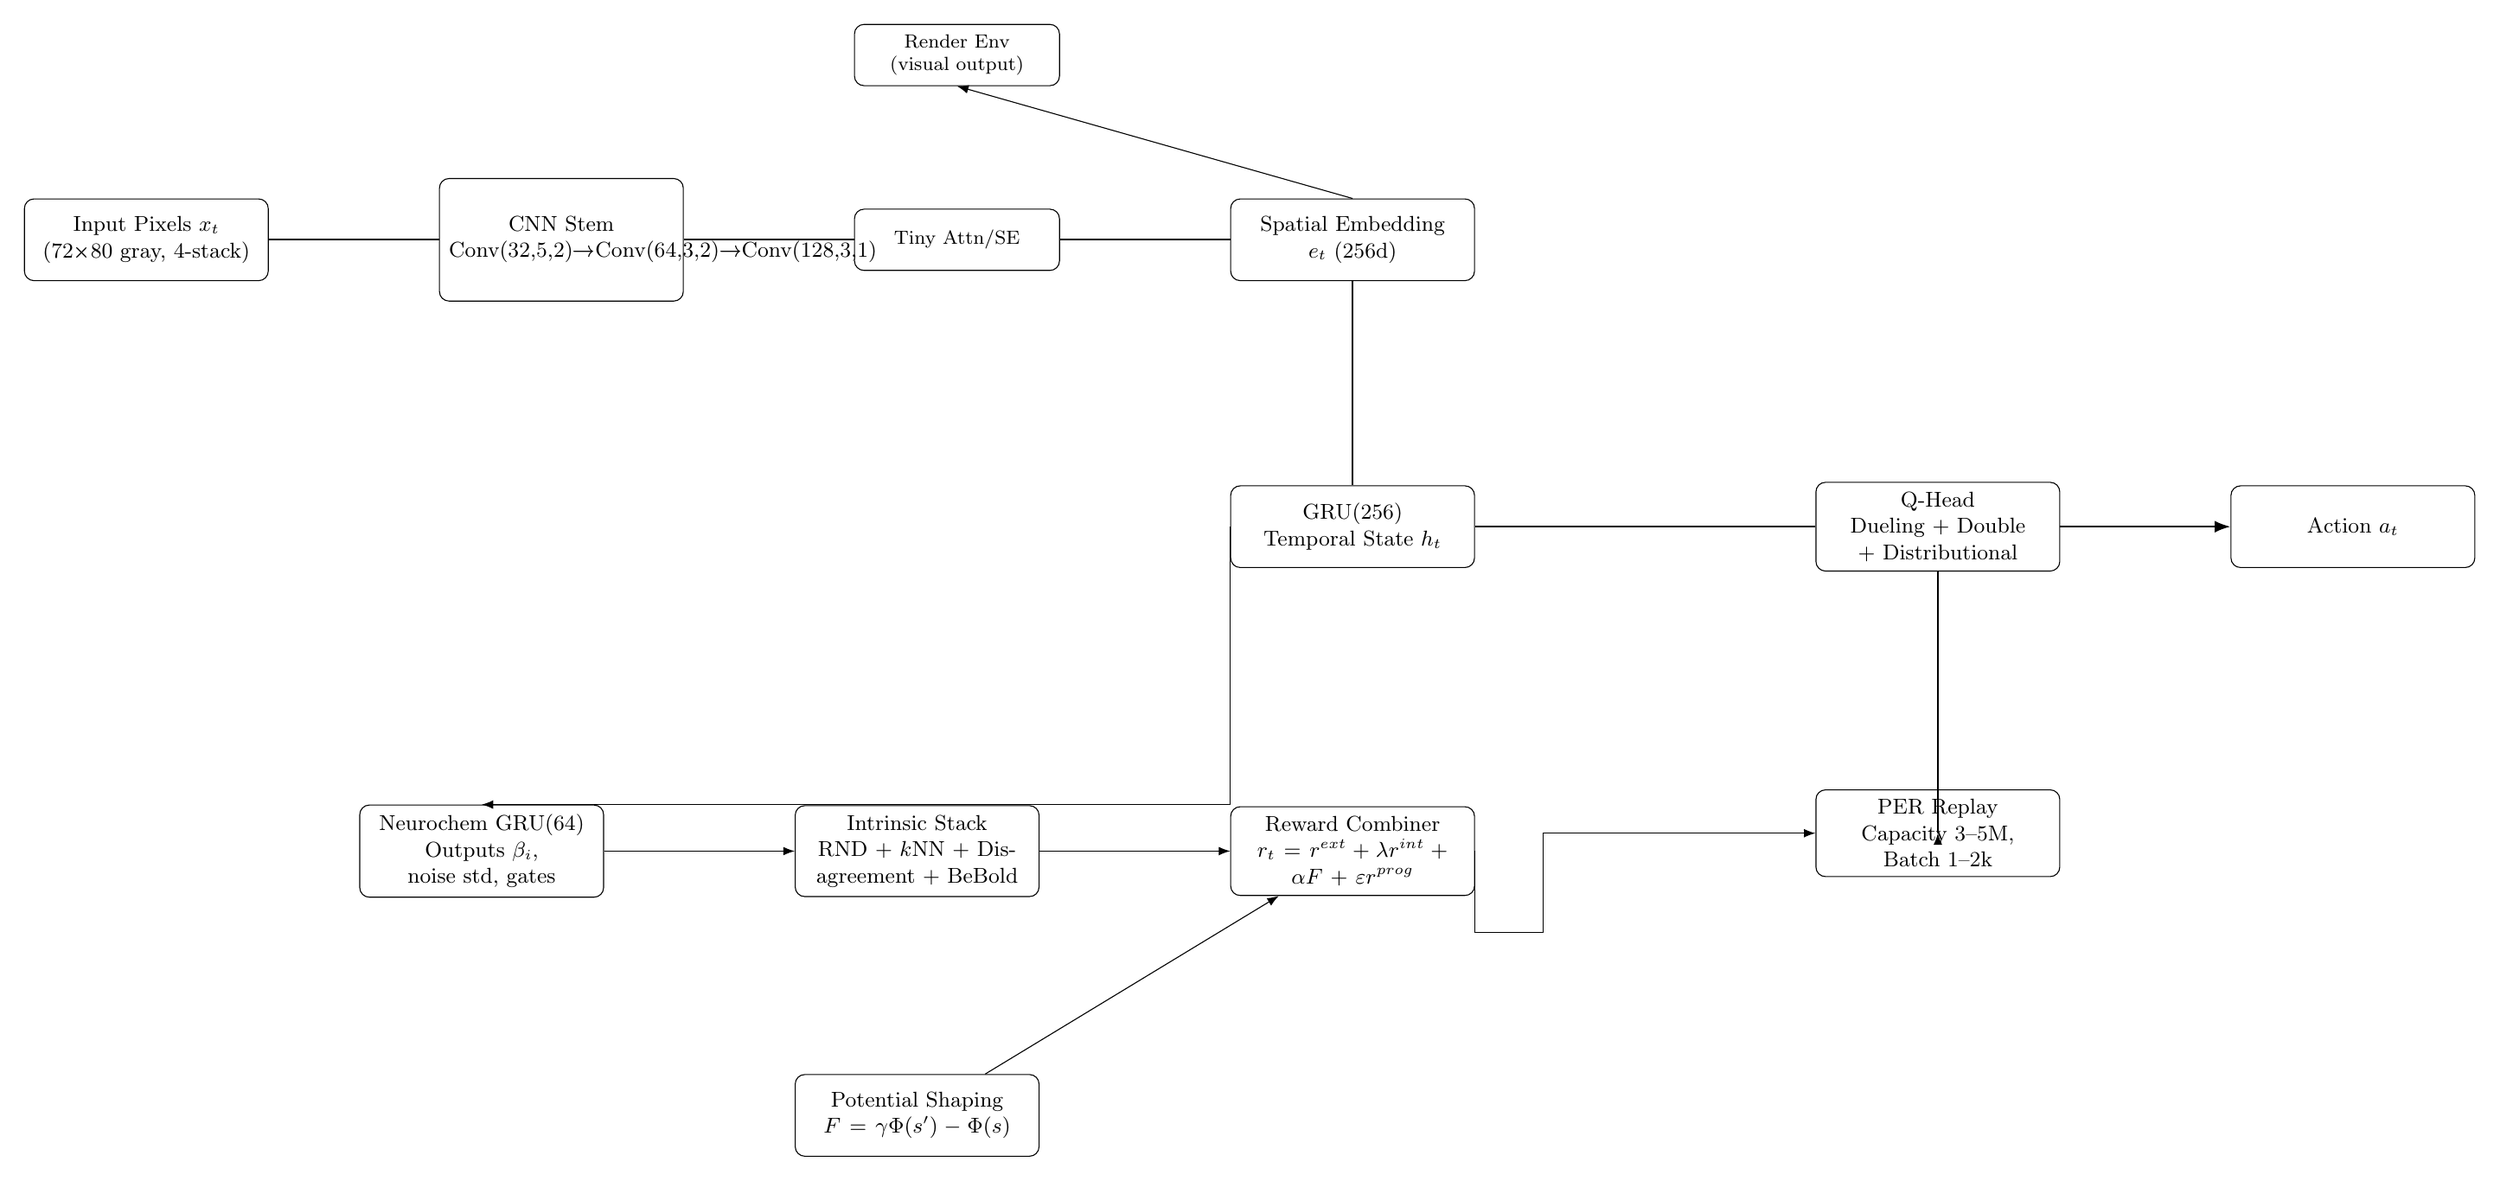
\begin{tikzpicture}[
  >=Latex,
  node distance=25mm and 22mm,
  box/.style={draw, rounded corners, align=center, font=\small,
              minimum height=12mm, text width=3.3cm, inner sep=4pt},
  tallbox/.style={draw, rounded corners, align=center, font=\small,
              minimum height=18mm, text width=3.3cm, inner sep=4pt},
  smallbox/.style={draw, rounded corners, align=center, font=\footnotesize,
                   minimum height=9mm, text width=2.8cm, inner sep=3pt}
]

\node[box] (pixels) {Input Pixels $x_t$\\(72×80 gray, 4-stack)};
\node[tallbox, right=25mm of pixels] (cnn) {CNN Stem\\Conv(32,5,2)→Conv(64,3,2)→Conv(128,3,1)};
\node[smallbox, right=25mm of cnn] (attn) {Tiny Attn/SE};
\node[box, right=25mm of attn] (embed) {Spatial Embedding\\$e_t$ (256d)};
\node[smallbox, above=18mm of attn] (render) {Render Env\\(visual output)};

\node[box, below=30mm of embed] (gru) {GRU(256)\\Temporal State $h_t$};
\node[box, right=50mm of gru] (qhead) {Q-Head\\Dueling + Double + Distributional};
\node[box, right=25mm of qhead] (act) {Action $a_t$};

\node[box, below=35mm of gru] (reward) {Reward Combiner\\$r_t = r^{ext} + \lambda r^{int} + \alpha F + \varepsilon r^{prog}$};
\node[box, below=32mm of qhead] (per) {PER Replay\\Capacity 3–5M, Batch 1–2k};

\node[box, left=28mm of reward] (intr) {Intrinsic Stack\\RND + $k$NN + Disagreement + BeBold};
\node[box, left=28mm of intr] (chem) {Neurochem GRU(64)\\Outputs $\beta_i$, noise std, gates};
\node[box, below=26mm of intr] (pot) {Potential Shaping\\$F = \gamma \Phi(s') - \Phi(s)$};

\draw[->, thick] (pixels) -- (cnn) -- (attn) -- (embed) -- (gru) -- (qhead) -- (act);
\draw[->] (qhead) |- (per);
\draw[->] (gru.west) |- (chem.north);
\draw[->] (chem) -- (intr);
\draw[->] (intr) -- (reward);
\draw[->] (pot) -- (reward);
\draw[->] (reward.east) |- ++(10mm,-12mm) |- (per.west);
\draw[->] (embed.north) -- (render.south);

\end{tikzpicture}}
\caption{High-level architecture with intrinsic motivation and neurochemical modulation.}
\end{figure}

\section{Algorithm (Optional Figure)}

\begin{figure}[H]
\centering
\begin{minipage}{0.48\linewidth}
\small
\begin{algorithm}[H]
\DontPrintSemicolon
\caption{Actor Loop}
Initialize env and episodic memory.\;
\For{$t = 0,1,2,\dots$}{
    Encode $x_t \to e_t \to h_t$ (CNN + GRU)\;
    Compute intrinsic signals at cadence $k_{\text{int}}$;\;
    Update $z_t$ via neurochem GRU; adjust $\beta_i$ and exploration noise;\;
    $Q_t \leftarrow$ Dueling+Double+Distributional head;\;
    Select $a_t$ using NoisyNet/$\epsilon$-greedy; step env;\;
    $F_t = \gamma\Phi(s')-\Phi(s)$ (normalized RND);\;
    $r_t = r^{ext}_t + \lambda r^{int}_t + \alpha F_t + \varepsilon r^{prog}_t$;\;
    Push $(s_t,a_t,r_t,s_{t+1},done)$ into PER.\;
}
\end{algorithm}
\end{minipage}\hfill
\begin{minipage}{0.48\linewidth}
\small
\begin{algorithm}[H]
\DontPrintSemicolon
\caption{Learner Loop}
\For{each update step}{
    Sample batch from PER;\;
    Build $n$-step distributional targets;\;
    $\mathcal{L}_Q \leftarrow$ Huber loss; apply soft target update ($\tau$);\;
    Add $\mathcal{L}_{\text{RND}}$ / auxiliary bonuses as needed;\;
    Update $\theta \leftarrow \theta - \alpha\nabla_\theta \mathcal{L}$ (AdamW);\;
    Refresh PER priorities and archive frontier states.\;
}
\end{algorithm}
\end{minipage}
\caption{Actor–learner loops showing intrinsic curiosity, neurochemical modulation, and prioritized replay.}
\end{figure}

\vfill
\begin{center}
    \rule{0.4\linewidth}{0.4pt}\\[0.5em]
    End of Proposal
\end{center}

\end{document}
